\documentclass[a4paper, 12pt]{article}

\usepackage[brazilian]{babel}
\usepackage{ae,aecompl}
\usepackage[utf8]{inputenc}

\usepackage{fullpage}  
\usepackage{indentfirst}      % Indenta o primeiro paragrafo das sections
\usepackage{graphicx}         % Utilizado para inserir imagens
\usepackage{hyperref}         % Cria link entre o sumario e as sections
\usepackage{fancyhdr}         % Permite alterar o header e footer
\usepackage{mdwlist}          % Permite criar listas com menos espaçamento
\usepackage[includefoot]{geometry}

% Seta o estilo padrao
\pagestyle{fancy}

% Configura links
\hypersetup{colorlinks=true,linkcolor=black,citecolor=black}

% Seta espacamento
\addtolength{\parskip}{2mm}
\addtolength{\footskip}{15mm}

% Coloca no pé a pagina atual
\begin{document}

% Inclua as variáveis
\newcommand{\titulo}{Documento de Projeto}
\newcommand{\subtitulo}{Produto: DIGI-DOC}
\newcommand{\autor}{Sérgio Oliveira Campos}
\newcommand{\data}{05 de Maio de 2008}
\newcommand{\cidade}{Brasília}

% Numero do contrato caso seja consultor
\newcommand{\ncontrato}{1234567890-32}


% Inclua header
\lhead {
	\setlength{\unitlength}{5mm} 
	\begin{picture}(0,0) 
		
\includegraphics[scale=0.75]{img/header.pdf} 
	\end{picture} 
	\textsf{\vspace{1cm}}
}

\chead{}
\rhead{}
\renewcommand{\headrulewidth}{0pt}


% Inluia a capa
\newpage
\textsf{\vspace{7.5cm}}
\begin{center}
	\noindent
	\huge{
		\textbf{\titulo}
	} \\
	\Large{
		\textbf{\subtitulo}
	}

	\vspace{8cm}

	\large{
		\textbf{\autor}\\
		\textsf{Contrato N$^{\circ}$: \ncontrato}\\
	}
\end{center}
\cfoot{\large{\cidade, \data}}


% Seta o footer das paginas iniciais para numeros Romanos
\cfoot{\thepage}
\setcounter{page}{1}
\pagenumbering{Roman}

% Sum√°rio
\newpage
\tableofcontents

% Lista de figuras
\newpage
\listoffigures

% Lista de tabelas
\newpage
\listoftables

% Seta o footer das paginas para numeros convencionais
\clearpage
\setcounter{page}{1}
\pagenumbering{arabic}

% PARA INSERIR NOVAS PAGINAS BASTA ADICIONAR AQUI:
% Conte√∫do
\section{Introdução}
\label{sec:intro}

Durante a primeira fase da elaboração do projeto {\it webscan}, foram realizadas as seguintes atividades:

\begin{description}
    \item[Casos de uso: ] Nessa atividade, descrita na seção \ref{sec:casos_de_uso}, foram elaborados diagramas de casos de uso, representando as principais interações entre atores e o sistema. Também foram elaborados os casos de uso completo-abstrato, de forma a dar detalhamento a cada caso de uso contido no diagrama;
    \item[Modelagem de dados: ] A modelagem de dados do projeto foi realizada para dar uma visão geral dos dados que serão tratados, e, como eles se relacionam entre si. A seção \ref{sec:modelo_de_dados} apresenta o resultado obtido desse trabalho realizado. 
    \item[Interface: ] Para essa atividade, descrita com mais detalhes na seção \ref{sec:mockups}, foram elaboradas as candidatas às telas de interface do sistema ({\it mockups} e também o curso de ações que um usuário pode realizar {\it storyboards};
    \item[Elaboração dos {\it Web Services}: ] Essa atividade consistiu na
        espeficação dos métodos que compõe a interface de comunicação da
        aplicação com outros sistemas. Toda a especificação está disponível
        na seção \ref{sec:web_services}. 
    \item[Pesquisa de bibliotecas: ] Essa atividade (apresentada nas seções \ref{sec:pesquisa_libs} e \ref{sec:pesquisa_ocr}) consistiu na realização de uma pesquisa sobre as bibliotecas de digitalização e de reconhecimento de textos respectivamente.

\end{description}

\subsection{Terminologia}

\subsubsection{Atividade de Desenvolvimento}
Atividade de desenvolvimento se refere à quantidade de escritas (ou seja, código sendo atualizado/adicionado) em um sistema de controle de versões, quando disponível.

\begin{description}
    \item[Alta:] diversas atividades no último mês.
    \item[Baixa:] algumas atividades ao longo dos últimos 3 meses.
    \item[Parado:] não houve nenhuma atividade de escrita nos últimos 6 meses.
\end{description}

\subsubsection{OCR - Optical Character Recognition}

O OCR (Optical Character Recognition), ou Reconhecimento Óptico de Caracteres, 
é a tecnologia responsável pela obtenção de texto apartir de uma imagem. Durante
este projeto a tecnologia será empregada para gerar documentos indexáveis\footnote{Documentos indexáveis: Que
podem ser encontrados pelo sistema de busca}.

\subsubsection{JSON}
Algumas vezes é necessário que uma pequena informação seja transmitida entre aplicações, e o formato XML acaba
burocratizando demasiadamente este processo. Outro cenário é o de múltiplas requisições em um curto espaço de
tempo, que leva o cliente e o servidor a uma sobrecarga para executar o \emph{parser}, além de um uso de
excessivo da banda para a transmissão dos dados.

A padronização de um formato Javascript para a transferencia de dados poderia ser uma alternativa para
solucionar estes problemas, e foi por isso que no ano de 2002 \emph{Douglas Crockford}, engenheiro da
\emph{Yahoo! Inc} propôs o formato JSON.

O principal objetivo era criar um padrão para troca de dados utilizando código javascript, ou seja, em forma
textual, gerando o mínimo de texto possível, o que tornaria o formato leve e ao mesmo tempo fácil de ser
interpretado pelo navegador. Para isso algumas assertivas foram seguidas:

\begin{itemize}
    \item Não poderia ser uma linguagem de marcação;
    \item Não seria um formato de documento;
    \item Não permitiria a representação de funções;
    \item Não permitiria a representação de estruturas cíclicas.
\end{itemize}

No ano de 2006 o formato foi oficializado pelo \emph{Network Working Group} e apresentado oficialmente a
comunidade durante a conferencia \textbf{XML 2006}.

O padrão apresentado é basicamente composto de um objeto (Figura \ref{fig:json_obj}) que possuí uma \emph{string}
descritiva e o seu valor, onde o seu valor pode assumir os formatos:

\begin{itemize}
    \item \emph{String}
    \item Número
    \item Vetor
    \item Objeto
    \item true, false e null
\end{itemize}

\begin{figure}[ht]
\begin{center}
\scalebox{0.6} {
    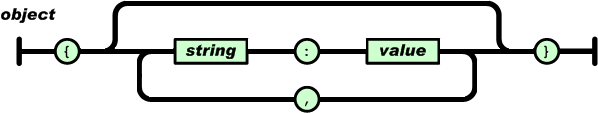
\includegraphics{img/json_obj.png}}
\end{center}
  \caption{Objeto JSON}
  \label{fig:json_obj}
\end{figure}

As definições detalhadas de cada um dos tipos e exemplos de código podem ser encontrados no site
http://www.json.org/.

\subsubsection{Web Services}

A W3C \footnote{http://www.w3c.org/} define \emph{web services} como um padrão que provê a
interoperabilidade entre duas aplicações de software, rodando sob diferentes plataformas e/ou
frameworks.
A interoperabilidade fornecida pelos \emph{web services} é disponibilizada por meio de funções
ou mesmo objetos na web, de forma que estes possam ser chamados através de um \emph{HTTP
request} e sua resposta retornada através de um \emph{HTTP response}.
Para que uma aplicação consiga se comunicar com a outra é necessário que ela conheça
e entenda o formato de entrada e saída de dados; para isso, costuma ser utilizado XML ou JSON.
Outro problema é que a aplicação deve saber qual o tipo de dados de um determinado
valor que chega a ela, e como ela implementa este valor. Este problema pode ser resolvido
de formas distintas; uma delas é a especificação trazer as informações necessárias; a outra
é o uso de um arquivo que trás esse tipo de informação, te tal forma que a aplicação
apenas leia este arquivo e faça as conversões necessárias. 



\section{Casos de Uso}
\label{sec:casos_de_uso}

Para o projeto, foram elaborados casos de uso do sistema. Na figura \ref{fig:casos_de_uso}
tem-se o diagrama de casos de uso. Na seção \ref{sec:casos_completos} tem-se os casos de uso
completo-abstrato, que indicam as principais atividades que acontecem em cada caso de uso, presentes no diagrama da figura \ref{fig:casos_de_uso}.

\subsection{Diagrama de Casos de Uso}
\begin{figure}[ht]
 \centering
  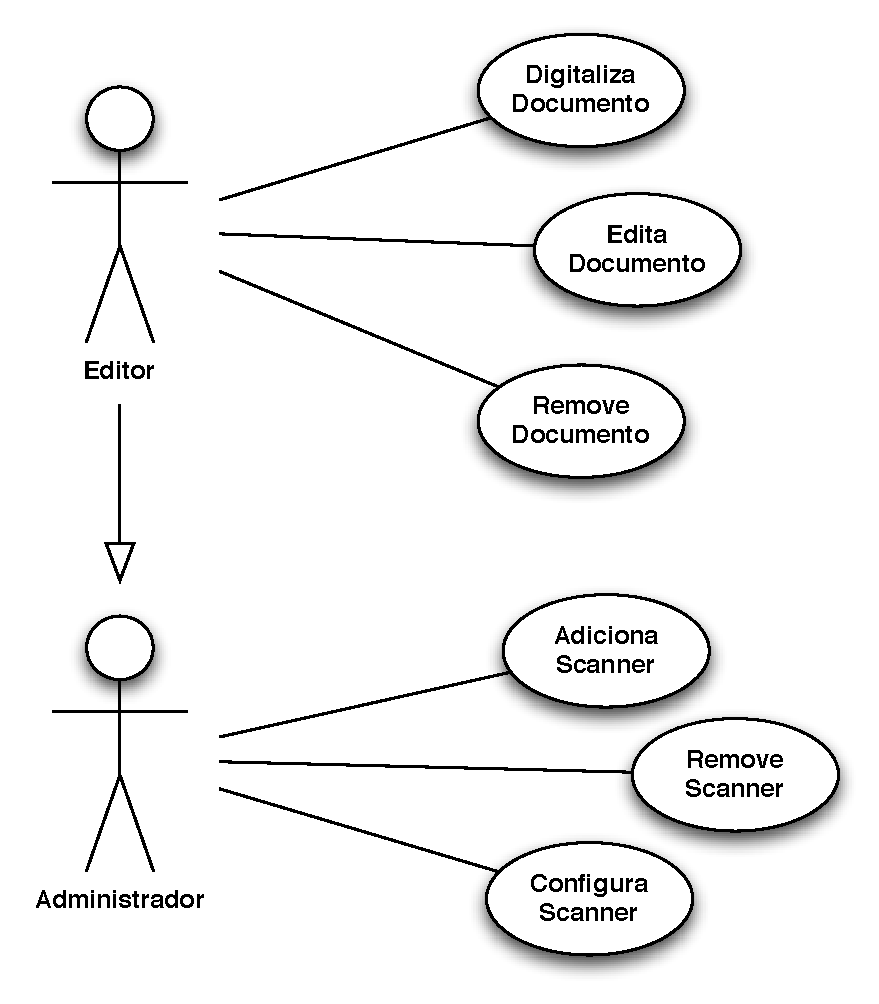
\includegraphics[scale=0.7]{img/use-case-diagram.pdf}
  \caption {Diagramas de casos de uso}
  \label{fig:casos_de_uso}
\end{figure}

\subsection{Casos de Uso Completos}
\label{sec:casos_completos}

\subsubsection{Caso de Uso: Digitaliza Documento}

\paragraph{Descrição:}
Nesse caso de uso o ator tem como função colocar um documento no {\it scanner} para digitalizá-lo.

\paragraph{Pré-condições:}
\begin{enumerate}
    \item Há um documento no {\it scanner};
    \item O {\it scanner} está configurado corretamente;
    \item O {\it scanner} está ligado e funcionando corretamente;
\end{enumerate}

\paragraph{Pós-condições:} 
\begin{enumerate}
    \item O documento estará digitalizado;
    \item O documento estará indexado para busca;
\end{enumerate}

\paragraph{Cenário de sucesso:}
\begin{enumerate}
    \item O {\it scanner} já foi previamente configurado e está operando corretamente;
    \item O ator colocou um documento no {\it scanner};
    \item O ator ativa o procedimento de digitalização;
    \item O ator muda a página do documento;
    \item O ator realiza os passos 3 e 4 até que todo o documento esteja digitalizado;
    \item O ator decide um nome para o novo documento;
\end{enumerate}

\paragraph{Fluxos alternativos:}
\begin{description}
    \item 1. O {\it scanner} não foi configurado ou não está operando; 
    \item (2-8). O {\it scanner} deixa de operar; 
    \item (1-8). O ator desiste da operação; 
\end{description}

\newpage
\subsubsection{Caso de Uso: Edita Documento}

\paragraph{Descrição:} Nesse caso de uso o ator tem como função selecionar um documento no sistema para alterar suas características.

\paragraph{Pré-condições:}
\begin{enumerate}
    \item Há pelo menos um documento digitalizado;
\end{enumerate}

\paragraph{Pós-condições:} 
\begin{enumerate}
    \item O documento foi alterado;
\end{enumerate}
    
\paragraph{Cenário de sucesso:}
\begin{enumerate}
    \item O ator encontrou o documento;
    \item O ator alterou os dados do documento;
    \item O ator confirmou as alterações;
\end{enumerate}

\paragraph{Fluxos alternativos}
\begin{description}
    \item 1. Não há documentos digitalizados; 
    \item 3. O ator não confirmou as alterações;
\end{description}


\newpage
\subsubsection{Caso de Uso: Remove Documento}

\paragraph{Descrição:} Nesse caso de uso o ator tem como função selecionar um documento para ser removido do sistema.

\paragraph{Pré-condições:}
\begin{enumerate}
    \item Há pelo menos um documento digitalizado;
\end{enumerate}

\paragraph{Pós-condições:} 
\begin{enumerate}
    \item O documento foi removido do sistema;
\end{enumerate}
    
\paragraph{Cenário de sucesso:}
\begin{enumerate}
    \item O ator encontrou o documento;
    \item O ator acionou a remoção do documento;
    \item O ator confirmou a remoção do documento;
\end{enumerate}

\paragraph{Fluxos alternativos}
\begin{description}
    \item 1. Não há documentos digitalizados;
    \item 3. O ator não confirmou a remoção do documento;
\end{description}

\newpage
\subsubsection{Caso de Uso: Adiciona Scanner}
 
\paragraph{Descrição:} Nesse caso de uso o ator tem como função preencher os dados necessários para a adição de um novo {\it scanner} no sistema.

\paragraph{Pré-condições:}
\begin{enumerate}
    \item Há pelo menos um {\it scanner} conectado ao computador onde o sistema está instalado;
\end{enumerate}

\paragraph{Pós-condições:} 
\begin{enumerate}
    \item O novo {\it scanner} está configurado e pronto para uso;
\end{enumerate}

\paragraph{Cenário de sucesso:}
\begin{enumerate}
    \item O ator preencheu os dados do {\it scanner} corretamente;
    \item O sistema encontrou o {\it scanner} que o ator se referiu;
    \item O sistema registrou o novo {\it scanner};
\end{enumerate}

\paragraph{Fluxos alternativos}
\begin{description}
    \item 1. Os dados digitados pelo autor são inválidos; 
    \item 2. Não há {\it scanners} conectados ao computador;
\end{description}

\newpage
\subsubsection{Caso de Uso: Remove Scanner}

\paragraph{Descrição:} Nesse caso de uso o ator tem como função escolher um {\it scanner} para ser removido do sistema.

\paragraph{Pré-condições:}
\begin{enumerate}
    \item Há pelo menos um {\it scanner} registrado no sistema;
\end{enumerate}

\paragraph{Pós-condições:} 
\begin{enumerate}
    \item O {\it scanner} não estará mais registrado no sistema;
\end{enumerate}

\paragraph{Cenário de sucesso:}
\begin{enumerate}
    \item O ator escolheu o  {\it scanner} a ser removido;
    \item O ator confirmou a remoção do {\it scanner} do sistema;
\end{enumerate}

\paragraph{Fluxos alternativos}
\begin{description}
    \item 1. Não há {\it scanners} registrados no computador; 
    \item 2. O ator não confirmou a remoção do {\it scanner};
\end{description}

\newpage
\subsubsection{Caso de Uso: Configurar Scanner}

\paragraph{Descrição:} Nesse caso de uso o ator tem como função escolher um {\it scanner} e em seguida inserir novos dados sobre esse {\it scanner}.

\paragraph{Pré-condições:}
\begin{enumerate}
    \item Há pelo menos um {\it scanner} registrado no sistema;
\end{enumerate}

\paragraph{Pós-condições:} 
\begin{enumerate}
    \item O {\it scanner} estará configurado e pronto para usar;
\end{enumerate}

\paragraph{Cenário de sucesso:}
\begin{enumerate}
    \item O ator escolheu o  {\it scanner} a ser configurado;
    \item O ator configurou o {\it scanner};
    \item O ator confirmou os dados das novas configurações;
\end{enumerate}

\paragraph{Fluxos alternativos}
\begin{description}
    \item 1. Não há {\it scanners} registrados no computador;
    \item 2. As configurações supridas pelo ator não são válidas; 
    \item 3. O ator não confirmou as novas configurações do {\it scanner};
\end{description}



\section{Interface}
\label{sec:mockups}

Nesta seção será apresentadas as telas do sistema, tanto para digitalização de novos documentos quanto para a configuração de {\it scanners}. Na seção \ref{sec:mockups_digitalizar}, tem-se os passos para digitalizar um novo documento (storyboard) e as telas que o sistema apresentará para o usuário (mockups). Na seção seguinte (seção \ref{sec:mockups_configurar}), tem-se as telas para configuração de {\it scanners}.

%%%%%%%%%%%%%%%%%%%%%%%%%%%%%%%%%%%%%%%%%%%%%%%%%%%%%%%%%%%%%%%%%%%
\subsection{Digitalizar Documento}
\label{sec:mockups_digitalizar}

Ao iniciar o sistema, o usuário é apresentado com a tela na figura \ref{fig:dig_1}. É interessante destacar o aviso no topo da tela, mostrando que o sistema está procurando por {\it scanners} instalados e configurados no sistema.

\begin{figure}[h]
 \centering
    \setlength\fboxsep{0pt}
    \setlength\fboxrule{0.5pt}
    \fbox{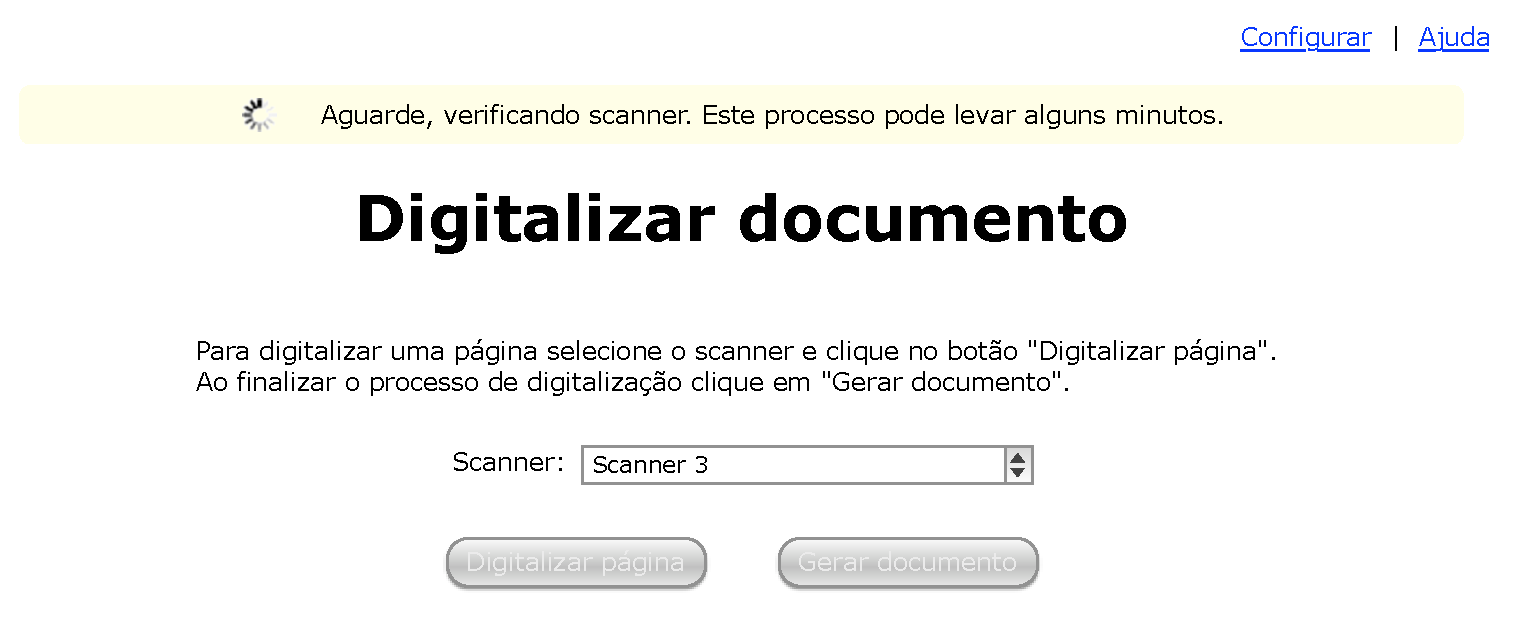
\includegraphics[scale=0.6]{img/mockups/digitalizacao-1.pdf}}
  \caption {Tela inicial do sistema}
  \label{fig:dig_1}
\end{figure}

Caso não haja nenhum {\it scanner} configurado no sistema, um aviso é apresentado ao usuário, pedindo a ele configure o {\it scanner} selecionado para ser usado pelo sistema.

\begin{figure}[h]
 \centering
    \setlength\fboxsep{0pt}
    \setlength\fboxrule{0.5pt}
    \fbox{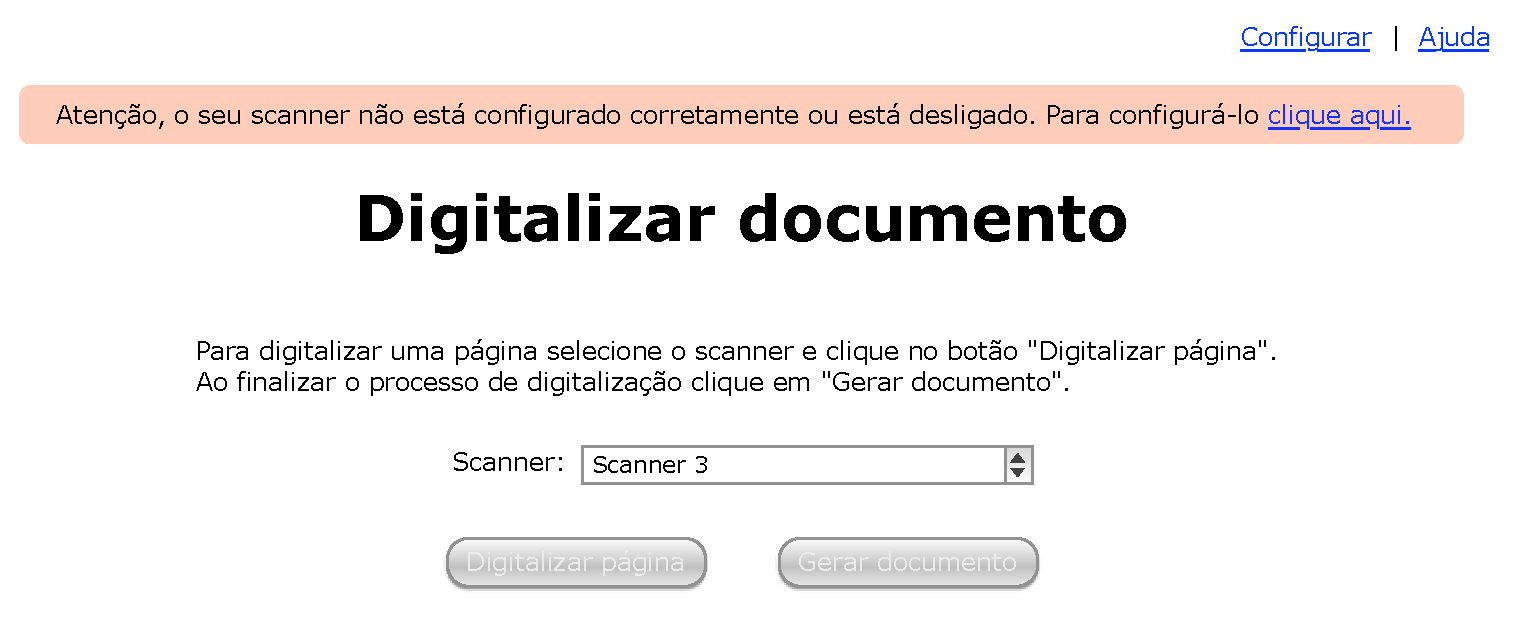
\includegraphics[scale=0.6]{img/mockups/digitalizacao-2.pdf}}
  \caption {Tela indiciando erro: o {\it scanner} selecionado não está corretamente configurado ou não está ligado}
  \label{fig:dig_2}
\end{figure}

Se o {\it scanner} estiver corretamente configurado e ligado, o usuário pode iniciar a criação de um novo documento, clicando no botão ``Digitalizar página'', apresentado na figura \ref{fig:dig_3}. Nessa situação, o botão ``Gerar documento'' está desativado e emite uma mensagem caso o usuário tente clicá-lo.

\begin{figure}[h]
 \centering
    \setlength\fboxsep{0pt}
    \setlength\fboxrule{0.5pt}
    \fbox{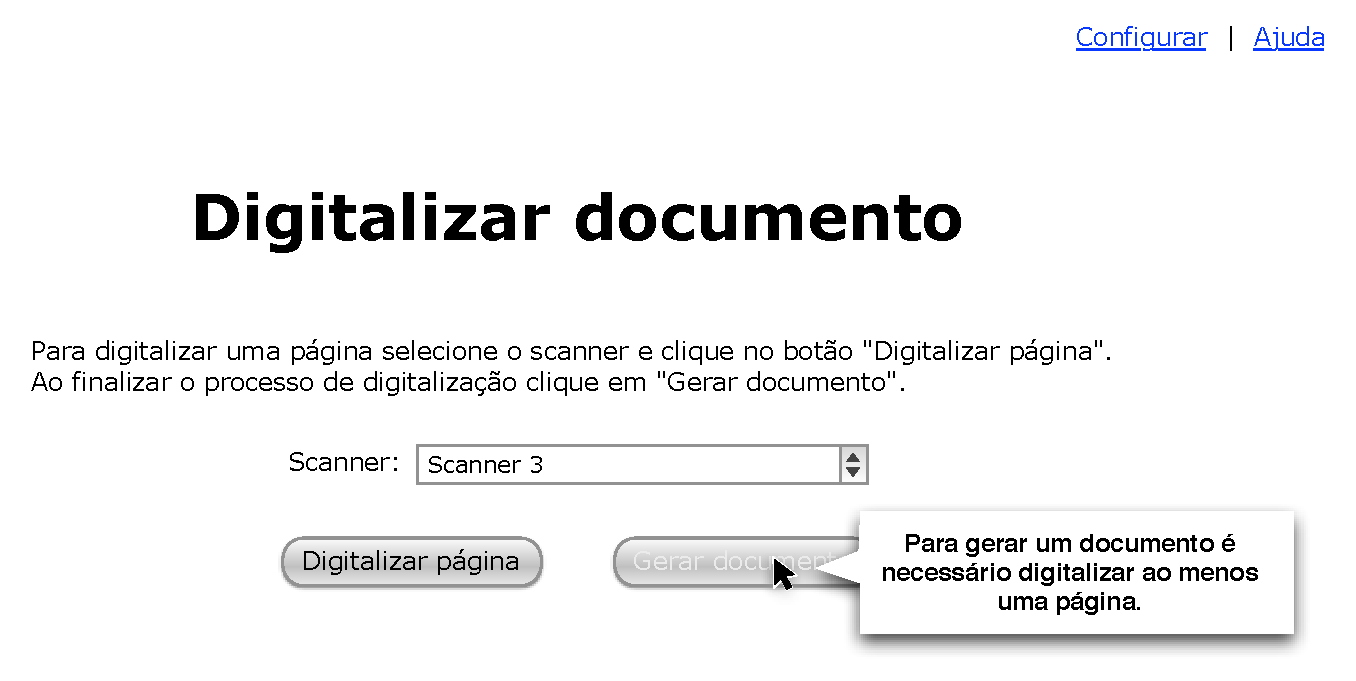
\includegraphics[scale=0.6]{img/mockups/digitalizacao-3.pdf}}
  \caption {Tela indicando o sistema está pronto e o usuário pode começar a digitalizar documentos}
  \label{fig:dig_3}
\end{figure}

Após clicar no botão ``Digitalizar página'', o é apresentada para o usuário uma mensagem para que ele espere a digitalização do documento que está no {\it scanner}, na tela apresentada na figura \ref{fig:dig_4}.

\begin{figure}[h]
 \centering
    \setlength\fboxsep{0pt}
    \setlength\fboxrule{0.5pt}
    \fbox{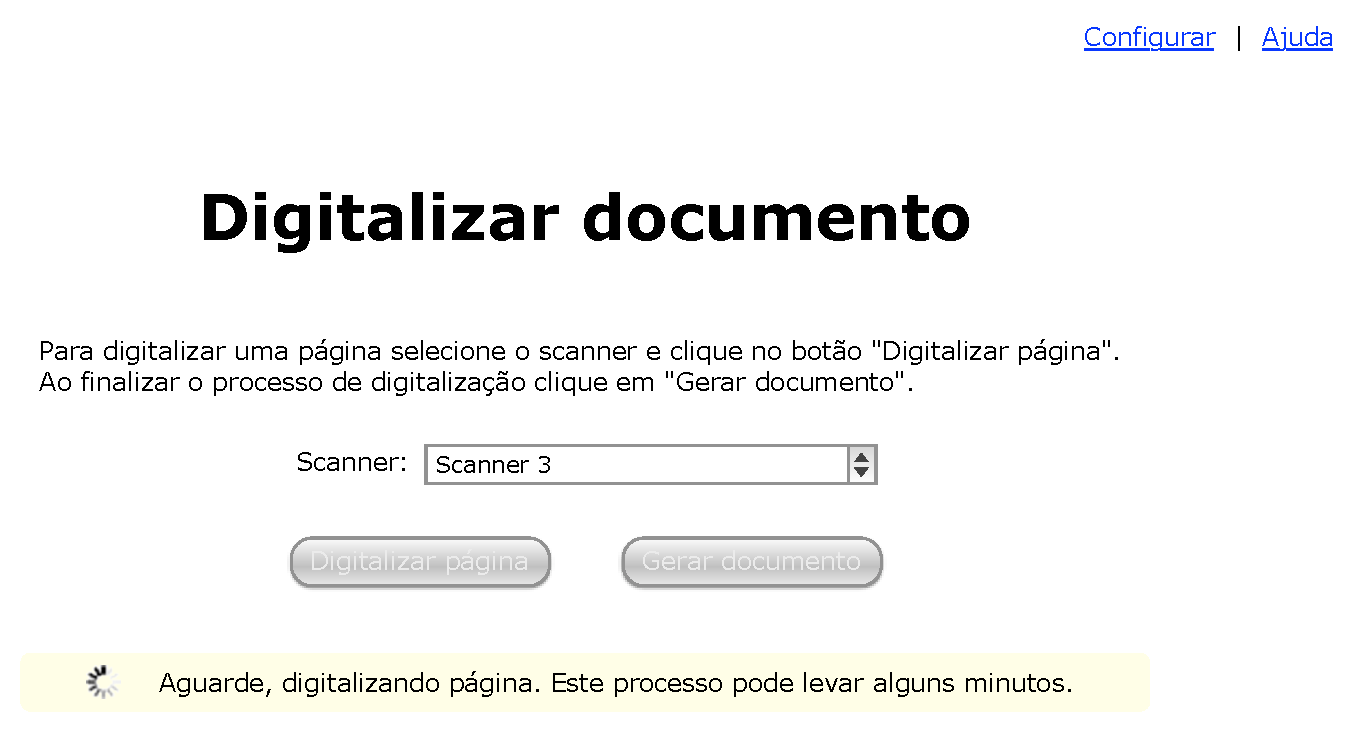
\includegraphics[scale=0.6]{img/mockups/digitalizacao-4.pdf}}
  \caption {Tela indicando que uma página está sendo digitalizada}
  \label{fig:dig_4}
\end{figure}

Em seguida, na figura \ref{fig:dig_5}, após a digitalização de várias páginas, é exibida pequenas amostras das páginas já digitalizadas e um marcador, indicando se a página deverá ser incluída no novo documento ou não. Após a seleção das páginas, o usuário deve clicar no botão ``Gerar documento''.

\begin{figure}[h]
 \centering
    \setlength\fboxsep{0pt}
    \setlength\fboxrule{0.5pt}
    \fbox{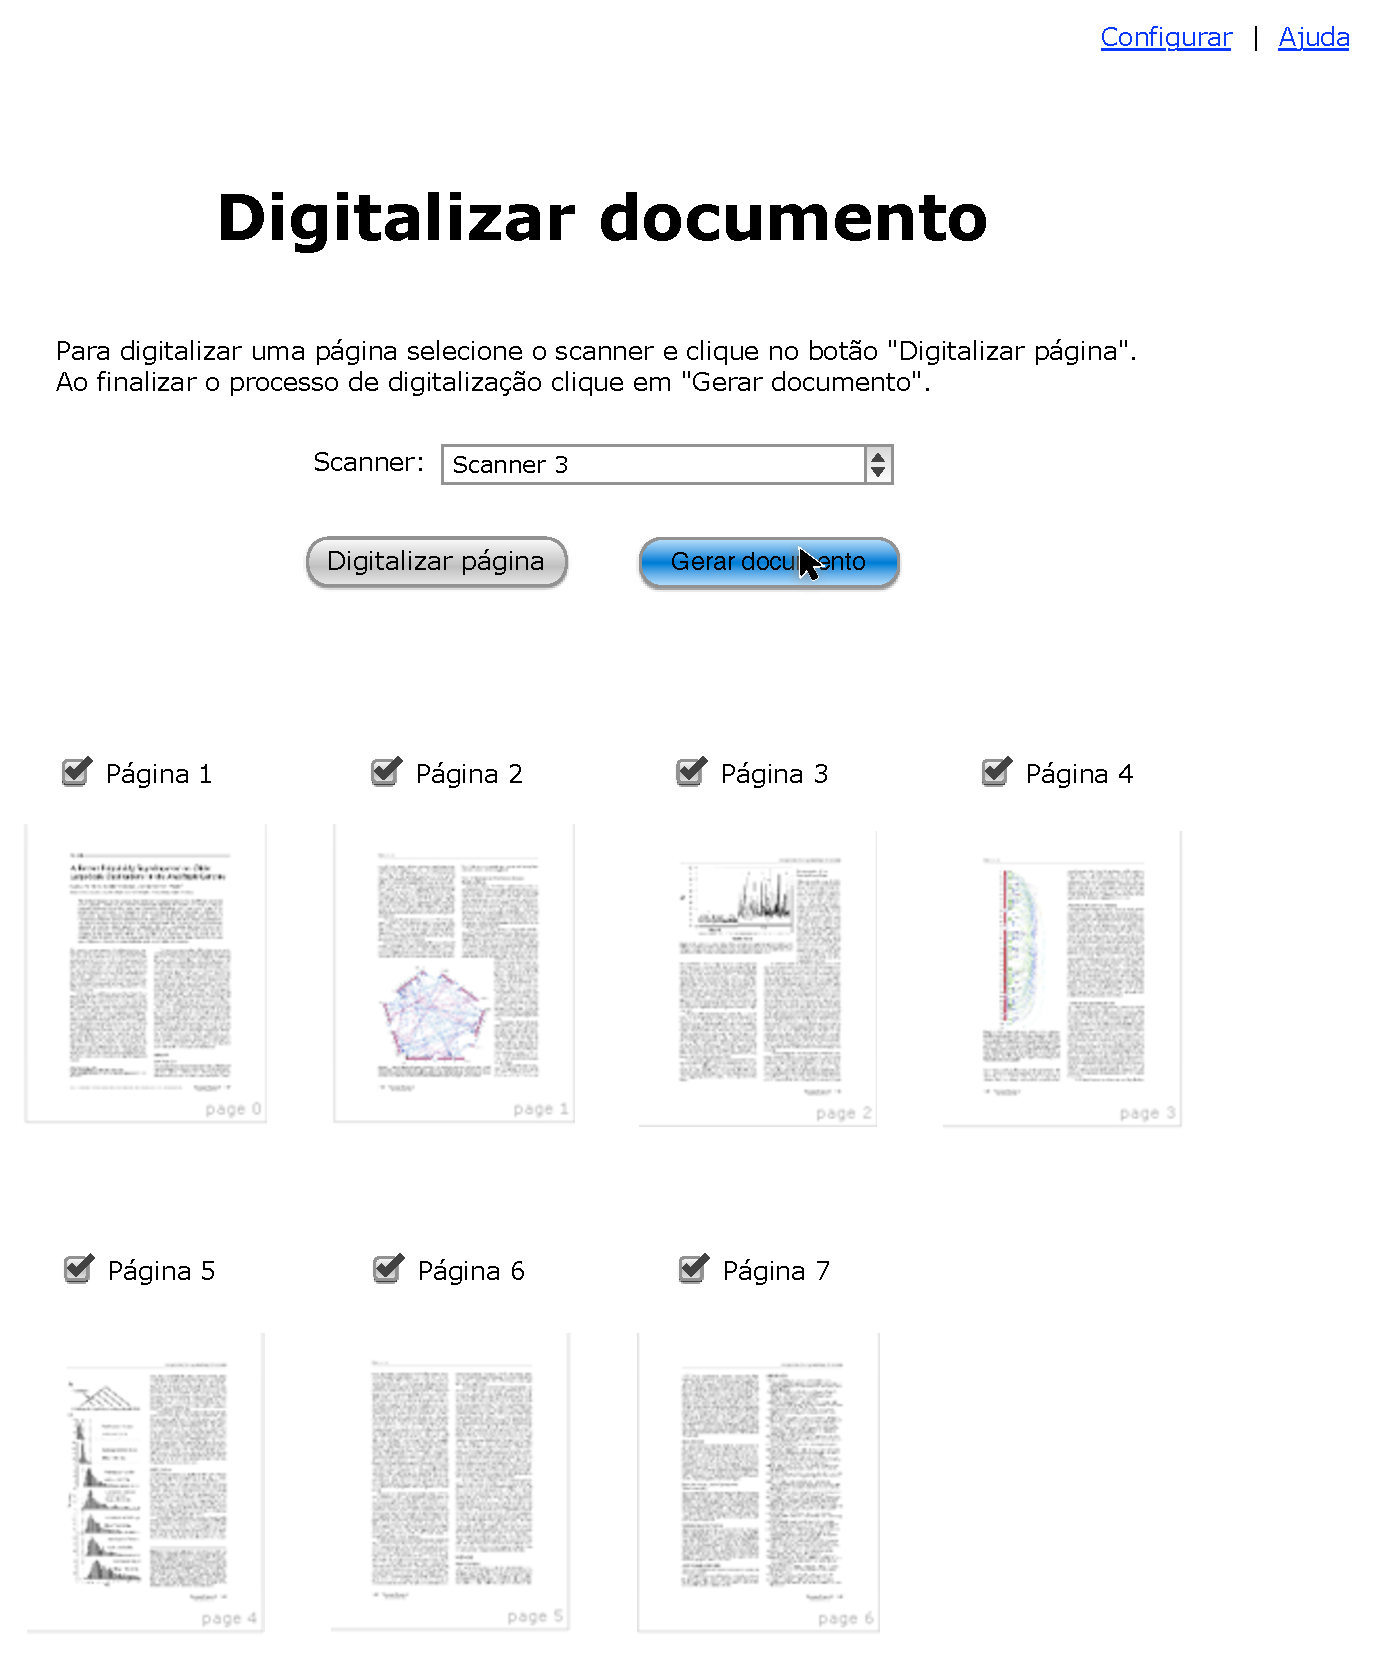
\includegraphics[scale=0.6]{img/mockups/digitalizacao-5.pdf}}
  \caption {Tela mostrando amostras das páginas já digitalizadas}
  \label{fig:dig_5}
\end{figure}

No próximo passo, representado pela figura \ref{fig:dig_6}, o usuário deve escolher então um nome para o documento e uma breve descrição sobre ele. A descrição deste novo documento é opcional.

\begin{figure}[h]
 \centering
    \setlength\fboxsep{0pt}
    \setlength\fboxrule{0.5pt}
    \fbox{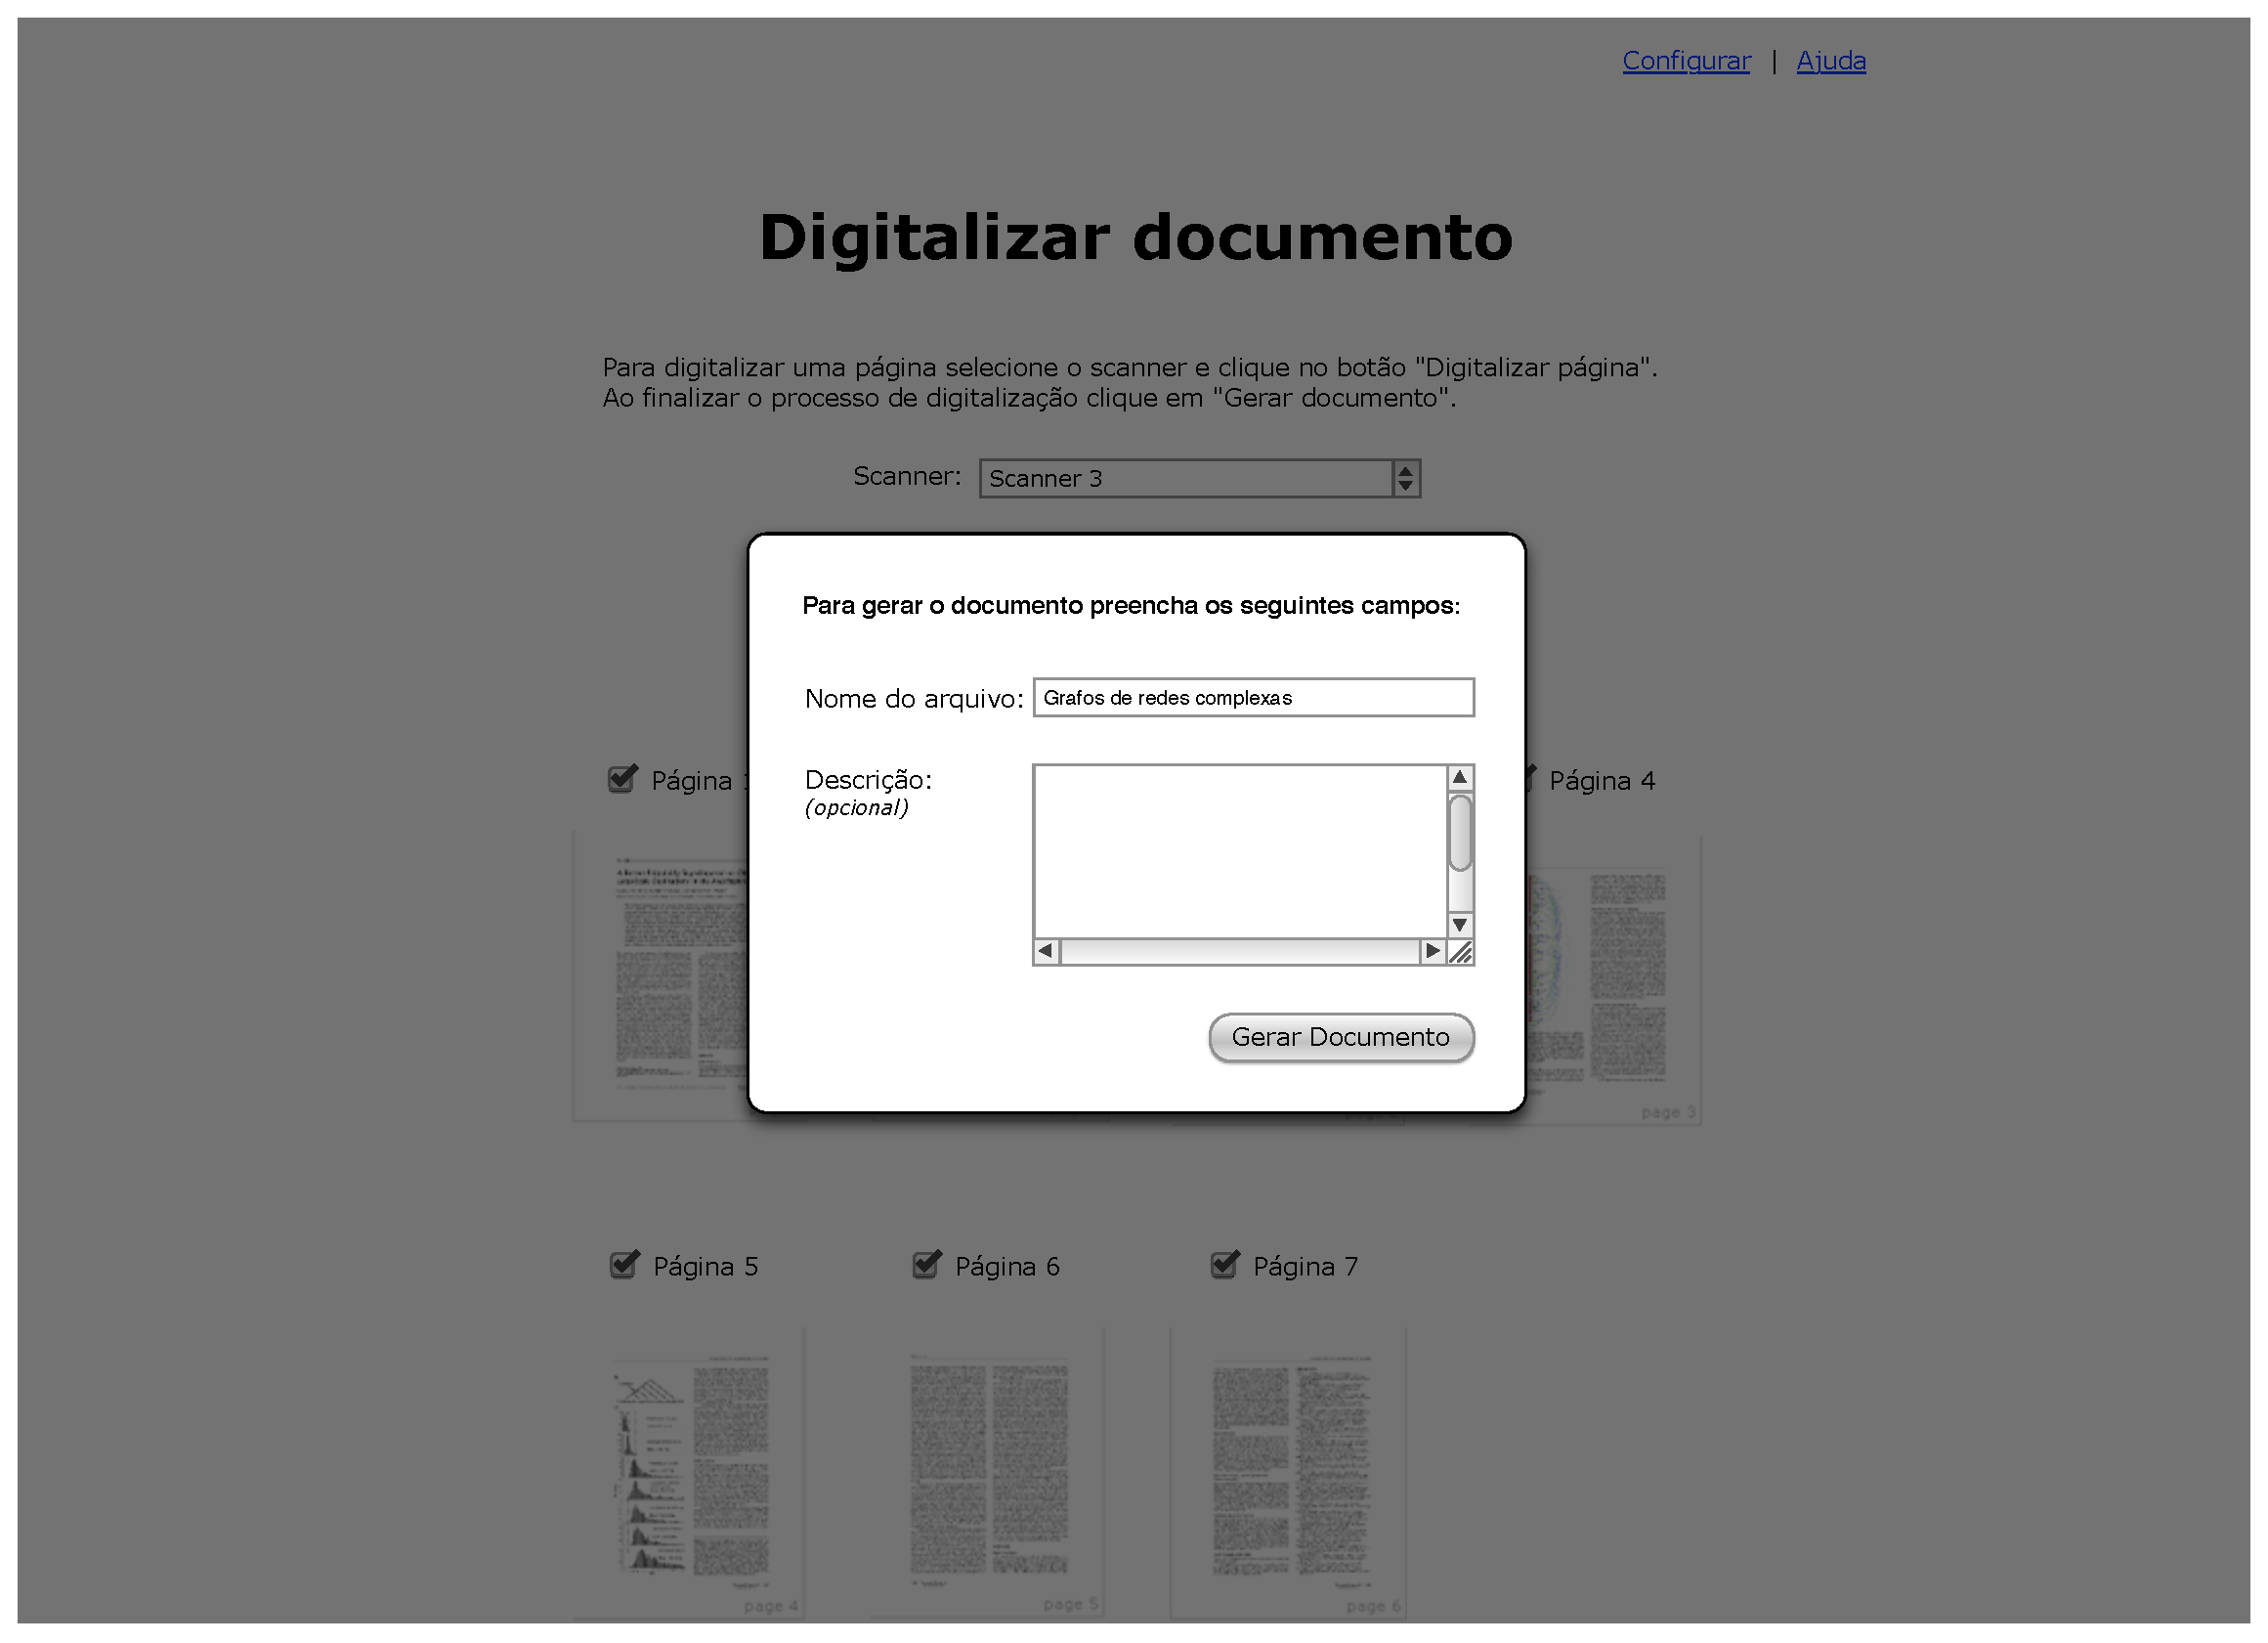
\includegraphics[scale=0.4]{img/mockups/digitalizacao-6.pdf}}
  \caption {Tela para a entrada de um nome e descrição para o novo documento}
  \label{fig:dig_6}
\end{figure}

Finalmente, após a criação do documento, o sistema mostra uma confirmação da criação do documento (figura \ref{fig:dig_7}) e indica seu estado. No exemplo, o sistema está pronto para digitalizar um novo documento.

\begin{figure}[h]
 \centering
    \setlength\fboxsep{0pt}
    \setlength\fboxrule{0.5pt}
    \fbox{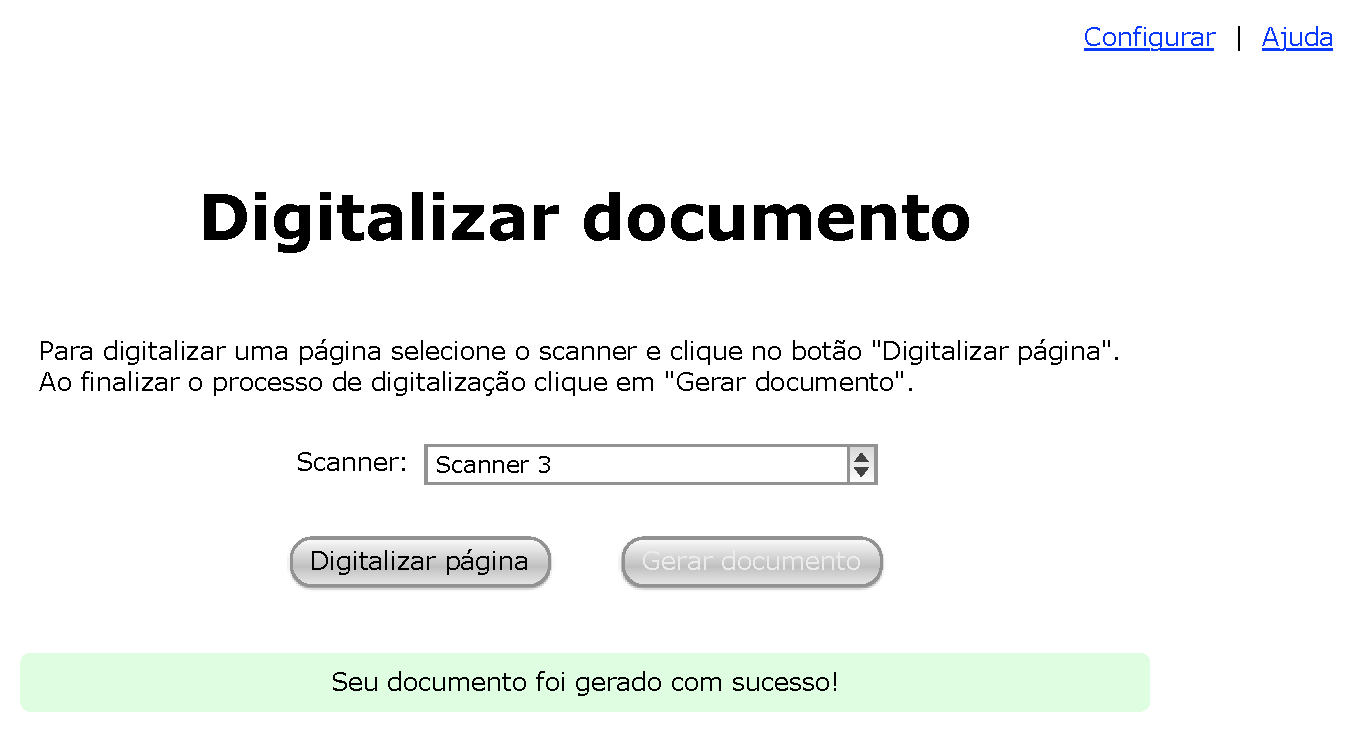
\includegraphics[scale=0.6]{img/mockups/digitalizacao-7.pdf}}
  \caption {Tela confirmando a criação de um novo documento}
  \label{fig:dig_7}
\end{figure}

A figura \ref{fig:dig_8} mostra a tela no caso em que o usuário digitalizou páginas anteriormente, porém não gerou um documento. Essas páginas ficam armazenadas no sistema e, logo que ele tente digitalizar novos documentos, poderá decidir se quer usar as páginas previamente digitalizadas ou descartá-las, para gerar um novo documento.

\begin{figure}[h]
 \centering
    \setlength\fboxsep{0pt}
    \setlength\fboxrule{0.5pt}
    \fbox{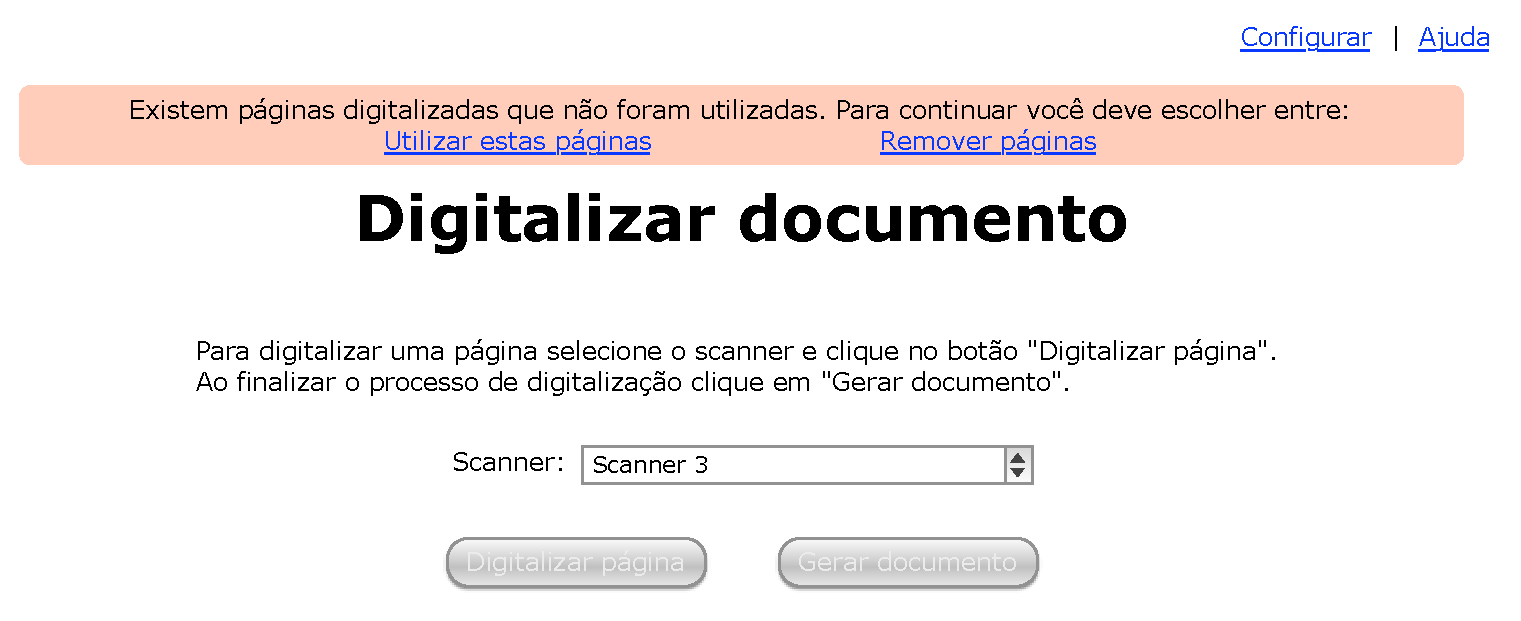
\includegraphics[scale=0.6]{img/mockups/digitalizacao-8.pdf}}
  \caption {Tela mostrando a situação de páginas previamente digitalizadas}
  \label{fig:dig_8}
\end{figure}



%%%%%%%%%%%%%%%%%%%%%%%%%%%%%%%%%%%%%%%%%%%%%%%%%%%%%%%%%%%%%%%%%%%%
\subsection{Configurar Scanner}
\label{sec:mockups_configurar}

Ao clicar no {\it link} ``Configurações'', o ususário deve selecionar qual {\it scanner} ele deseja configurar. Na tela \ref{fig:config_1}, é possível ver uma tela que mostra a escolha de um dispositivo para configuração.

\begin{figure}[h]
 \centering
    \setlength\fboxsep{0pt}
    \setlength\fboxrule{0.5pt}
    \fbox{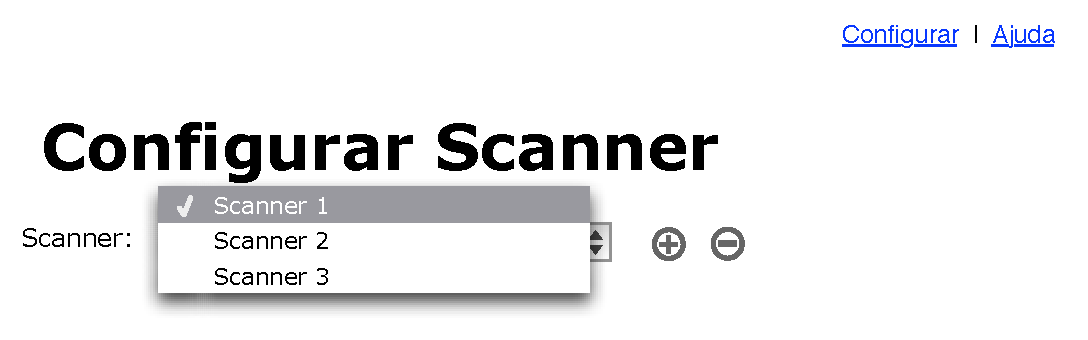
\includegraphics[scale=0.6]{img/mockups/config-1.pdf}}
  \caption {Tela mostrando a seleção de {\it scanners} para configuração}
  \label{fig:config_1}
\end{figure}

Após a escolha do {\it scanner}, o usuário encontra a tela exibida na figura \ref{fig:config_2}, na qual encontram-se campos para configuração do dispositivo, como tamanho da página, nome e modelo do {\it scanner}. É interessante notar os botões ``+'' e ``-'', para a adição e remoção de {\it scanners}, respectivamente.

\begin{figure}[h]
 \centering
    \setlength\fboxsep{0pt}
    \setlength\fboxrule{0.5pt}
    \fbox{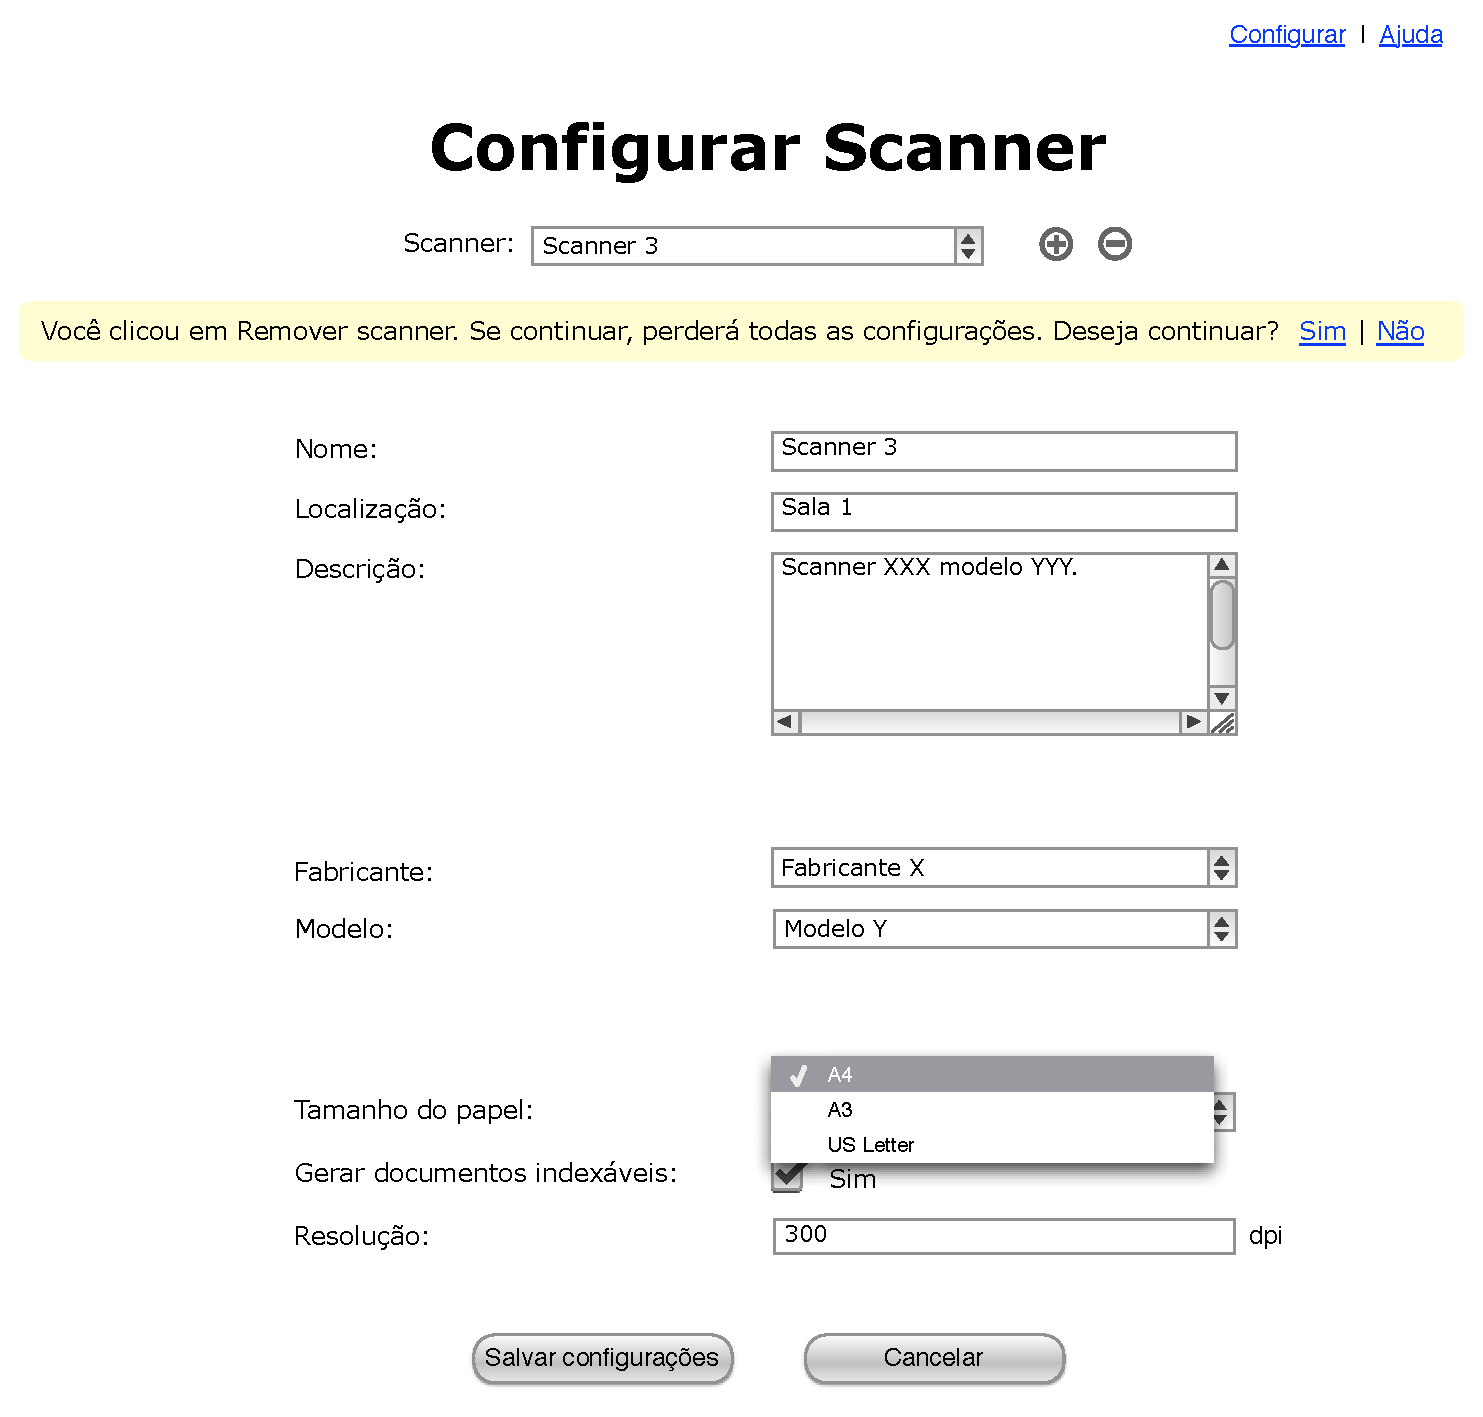
\includegraphics[scale=0.6]{img/mockups/config-2.pdf}}
  \caption {Tela mostrando as configurações de um {\it scanner}}
  \label{fig:config_2}
\end{figure}

\section{Bibliotecas de Digitalização}
\label{sec:pesquisa_libs}

Uma das atividades na fase atual do projeto foi elaborar uma pesquisa sobre as principais bibliotecas de digitalização de documentos disponíveis para plataformas Microsoft Windows, através da interface TWAIN e para plataforma GNU/Linux, através da interface SANE. 

Na seção \ref{sec:twain}, tem-se as principais bibliotecas encontradas para o uso da interface TWAIN e então, na seção \ref{sec:sane}, tem-se as principais bibliotecas encontradas para o uso da interface SANE.

\subsection{TWAIN}
\label{sec:twain}

\subsubsection{Descrição}
TWAIN é a interface de câmeras digitais e scanners específica para plataforma Windows 32 bits apenas. Não suporta scanners distribuídos na rede e não separa interface do driver (segundo www.sane-project.org).

\subsubsection{Bibliotecas}
\begin{description*}
	\item[Nome:] TWAIN Module
	\item[Linguagem(ns):] Python (versões 2.1 até 2.5)
	\item[Licença:] GPLv2
	\item[Plataforma(s):] Windows 32 bits
	\item[Endereço:] http://twainmodule.sourceforge.net
	\item[Última versão:] 1.0.3
	\item[Data da última atualização do site:] Novembro de 2006
	\item[Data do último {\it release}:] 31 de maio de 2007
	\item[Atividade de desenvolvimento:] parado
	\item[Descrição:] 
	Bem completa. Suporta atividades básicas TWAIN como funções prontas ou funções TWAIN avançadas que podem ser implementadas. Possui documentação ampla, com tutoriais, referências, guias e exemplos.
\end{description*}

\begin{description*}
	\item[Nome:] EZTwain
	\item[Linguagem(ns):] C, C++, Visual Basic, Delphi, entre outras
	\item[Licença:] Domínio público
	\item[Plataforma(s):] Windows 32 bits
	\item[Endereço:] http://www.dosadi.com/eztwain1.htm
	\item[Última versão:] 1.16
	\item[Data da última atualização do site:] Não disponível
	\item[Data do último {\it release}:] 11 de maio de 2007
	\item[Atividade de desenvolvimento:] parado
	\item[Descrição:] 
	É bastante popular, inclusive é amplamente usado através de um {\it wrapper} Java para TWAIN. Documentação limitada, porém possui exemplos prontos em C. Para C, foi testado apenas em Visual C++ 5 e 6.
\end{description*}

\begin{description*}
	\item[Nome:] TWAIN Development Kit
	\item[Linguagem(ns):] C, C++ (Visual Studio)
	\item[Licença:] Privada
	\item[Plataforma(s):] Windows 32 bits
	\item[Endereço:] http://www.twain.org
	\item[Última versão:] Não disponível
	\item[Data da última atualização do site:] Não disponível
	\item[Data do último {\it release}:] Não disponível
	\item[Atividade de desenvolvimento:] Não disponível
	\item[Descrição:] 
	Documentação esparsa, faltam exemplos
\end{description*}

%%%%%%%%%%%%%%%%%%%%%%%%%%%%%%%%%%%%%%%%%%%%%%%%%%%%%%%%%%%%%%%%%%%%%%%%%%%%%%%%%%%%%%%%%%%%%%%%%%%%%%%%%%%%%

\subsection{SANE}
\label{sec:sane}

\subsubsection{Descrição}
SANE (Scanner Access is Now Easy) é uma implementação de aquisição de imagens comum em sistemas open-source, como o Linux e FreeBSD. Há implementações para BeOS, OS/2 e MacOS X.

\subsubsection{Bibliotecas}

\begin{description*}
	\item[Nome:] SANE API
	\item[Linguagem(ns):] C
	\item[Licença:] GPL
	\item[Plataforma(s):] FreeBSD, Linux, BeOS, HP-UX, entre outros.
	\item[Endereço:] http://www.sane-project.org
	\item[Última versão:] 1.0.19
	\item[Data da última atualização do site:] Não disponível
	\item[Data do último {\it release}:] 11 de fevereiro de 2008
	\item[Atividade de desenvolvimento:] alta
	\item[Descrição:] 
	Documentação ampla, comunidade ativa, muitas implementações disponíveis para serem usadas como exemplos.
\end{description*}

\begin{description*}
	\item[Nome:] PIL (Python Imaging Library)
	\item[Linguagem(ns):] Python (versões 2.4 e 2.5)
	\item[Licença:] ver http://www.pythonware.com/products/pil/license.htm
	\item[Plataforma(s):] FreeBSD, Linux, BeOS, HP-UX, entre outros.
	\item[Endereço:] http://www.pythonware.com/products/pil/
	\item[Última versão:] 1.1.6
	\item[Data da última atualização do site:] Não disponível
	\item[Data do último {\it release}:] 3 de dezembro de 2006
	\item[Atividade de desenvolvimento:] Não disponível
	\item[Descrição:] 
	Amplamente usada para processamento de imagens em Linux, usada por diversos front-ends que usam python. Biblioteca simples, manual com tutorial incluso no código fonte da PIL.
\end{description*}




\clearpage

% Glossário
\section{Glossário}

\subsection{Atividade de Desenvolvimento:}
Atividade de desenvolvimento se refere à quantidade de escritas (ou seja, código sendo atualizado/adicionado) em um sistema de controle de versões, quando disponível.

\begin{description}
	\item[Alta:] diversas atividades no último mês.
	\item[Baixa:] algumas atividades ao longo dos últimos 3 meses.
	\item[Parado:] não houve nenhuma atividade de escrita nos últimos 6 meses.
\end{description}


\end{document}
